% !TeX spellcheck = pt_BR
%!TEX root = ../main_text.tex
\chapter{Princípios do Particionamento  de Sistemas Gerais} \label{chap:design}
    
    A seguir, serão descritos alguns tópicos seguindo conceitos estabelecidos pelo livro de \citet{Sass2010} e utilizado por vários trabalhos como \citet{Arato2003, Arato2005, Mann2007, BenHajHassine2017}.
    
    É possível descrever sistemas livre de especificações formais de \software\ ou \hardware\ por meio de descrição de protótipo simples, conhecidos como \Design\ de Referência de \Software\ (DRS).
    %Como será visualizado a seguir, sua vantagem mais notável é a generalização de uma especificação completa, eliminando quaisquer tipo de incertezas sobre o comportamento do sistema ao realizar uma análise sobre, sendo este podendo ser representado por diversas formas.
    % além de outras como o fato de que sua especificação pode ser analisada por ferramentas computacionais, e gerando modelos aut.
    %
    %Assumindo que o \design\ de referência de \textit{software} já exista,
    %Primeiramente, será demonstrado matematicamente como computação está em \design\ referencial de \sof%htware\ para que depois, isso possa nos auxiliar na decisão do que deverá ser implementado em nível de \hs.
    Como um algoritmo pode ser representado em forma de grafo de rotinas, pode-se então associar o \design\ da rotina com o uso da teoria de grafos \citep{Mann2007}, em especial o Gráfico de Controle de Fluxo (GCF).
    Ele é definido por
    \begin{equation}
        C = (B, F) \label{eq:subrotina}
    \end{equation}
    
    onde $B$ são vértices que representam tarefas constituídas de sub-rotinas $ b_i $
    %http://www.dcc.ufrj.br/~gabriel/microarq/Escalonamento.pdf
    e $ F $ são arestas que indicam a todas as possibilidades de caminhos entre as tarefas.
    
    
    A decomposição de um DRS pode gerar dois componentes sendo uma porção a ser realizada em \hardware\ e outra executada em \software.
    Essa de divisão é chamada de Particionamento \HS.
    %Segundo \citeauthor{Sass2010}, para sistemas em FPGA, o particionamento é um sub-problema de um problema mais geral no âmbito de \codesign, onde refere-se ao \design\ cooperativo entre engenheiros de \hs\ para um desenvolvimento mais eficiente.% envolvendo \textit{stakeholders}, por exemplo.
    %Para continuar, deve-se definir alguns conceitos básicos, descritos na Seção \ref{sec:gc}.
    
    \section{Definição Formal do Problema de Particionamento \HS} \label{sec:definicao_particionamento}
        
        Modelado as rotinas do \software\ utilizando o GCF, tem-se que o conjunto de GCF consiste em um Grafo de Chamada (GC), ou seja,
        %
        %\begin{equation}
        %    \mathcal{C} = {C_0, C_1, \dots C_{n-1}}
        %\end{equation}
        $ \mathcal{C} = {C_0, C_1, \dots C_{n-1}} $
        %
        %onde $ C_i = (V_i, E_i) $
        onde $ C_i = (B_i, F_i) $ representa o grafo de controle de fluxo de uma tarefa $ i $, como mostrado na Equação~\ref{eq:subrotina}.
        Sendo assim, o grafo estático de chamada da aplicação é descrito por
        %
        %\begin{equation}
        %    \mathcal{A} = (\mathcal{C}, \mathcal{L}) \label{eq:a}
        %\end{equation}
        $ \mathcal{A} = (\mathcal{C}, \mathcal{L}) \label{eq:a} $
        %
        onde \A\ representa uma aplicação específica e $ \mathcal{L} \subseteq \mathcal{C} \times \mathcal{C} $ é um subconjunto do plano cartesiano dos GCF.
        Duas tarefas são relacionadas se podem ser determinadas no tempo de compilação que a tarefas $ i $ tem potencial de invocar a tarefa $ j $, ou seja, $ (C_i, C_j) \in \mathcal{L} $.
       
        
        Conceitos básicos definidos, tem-se que uma partição $ \mathcal{S} = \{S_0, S_1, \dots S_i\} $ sendo $ i $ a quantidade de partições.
        Uma partição \Ss\ de um conjunto universal $ U $ é definida como um conjunto de subconjuntos de $ U $ sendo este o conjunto de todas as tarefa, ou seja
        %
        \begin{equation}
            \bigcup_{S \in \mathcal{S}} S = U \label{eq:part_form_1}
        \end{equation}
        \begin{equation}
            \forall S, S' \in \mathcal{S}\ |\ S \cap S' = \emptyset \label{eq:part_form_2}
        \end{equation}
        \begin{equation}
            \forall S \in \mathcal{S}\ |\ S \neq \emptyset \label{eq:part_form_3}
        \end{equation}
        %
        Descrevendo textualmente, a Equação \ref{eq:part_form_1} descreve que cada elemento de $ U $ é um membro de, pelo menos, um subconjunto $ S \in \mathcal{S} $ e as Equações \ref{eq:part_form_2} e \ref{eq:part_form_3} especifica que os subconjuntos $ S \in \mathcal{S} $ são emparelhados disjuntos e não vazio.
        Em outras palavras, cada elemento do nosso universo $ U $ termina exatamente em um dos subconjuntos de $\mathcal{S}$ e nenhum dos subconjuntos são vazios.
        
        \begin{comment}
        %exemplo
        Por exemplo, considerando um sistema hipotético \wearable\ na qual possui o universo $ U = \{a, e, i, o, u, y\} $ de recursos de processamento.
        Dessa forma, uma partição desse problema $ \mathcal{X}_a $ de $ U $ pode ser representado por
        %
        \begin{equation}
            \mathcal{X}_a = \left\{\{a, e, i, o, u\}, \{y\}\right\} \label{eq:xa}
        \end{equation}
        %
        e supondo que o conjunto possa ser representando por cada unidade, uma outra forma de representação pode ser
        %
        \begin{eqnarray}
            \mathcal{X}_b &=& \left\{\{a\}, \{e\}, \{i\}, \{o\}, \{u\}, \{y\}\right\} \label{eq:part_a} \\
            \mathcal{X}_c &=& \left\{\{a\}, \{e\}, \{i\}, \{o\} \right\} \label{eq:part_c} \\
            \mathcal{X}_d &=& \left\{\{a, e, i\}, \{i, o, u, y\}, \{\}\right\} \label{eq:part_d}
        \end{eqnarray}
        %
        Sobre tais conceitos, a Partição \ref{eq:part_c} viola a Equação \ref{eq:part_form_1} e a Partição \ref{eq:part_d} viola as Equações \ref{eq:part_form_2} e \ref{eq:part_form_3}, pois a primeira omite um item $y$ e a segunda possui um conjunto vazio além de redundância.
        %
        Assim, ao utilizar o particionamento para este exemplo, a Figura \ref{fig:parti_alfabeto} ilustra o $ \mathcal{X}_a $ (Equação \ref{eq:part_a}) graficamente, segundo a Partição \ref{eq:xa} como seria uma divisão entre \hs\ dos recursos listados.
        
        \begin{figure}[h] \centering
            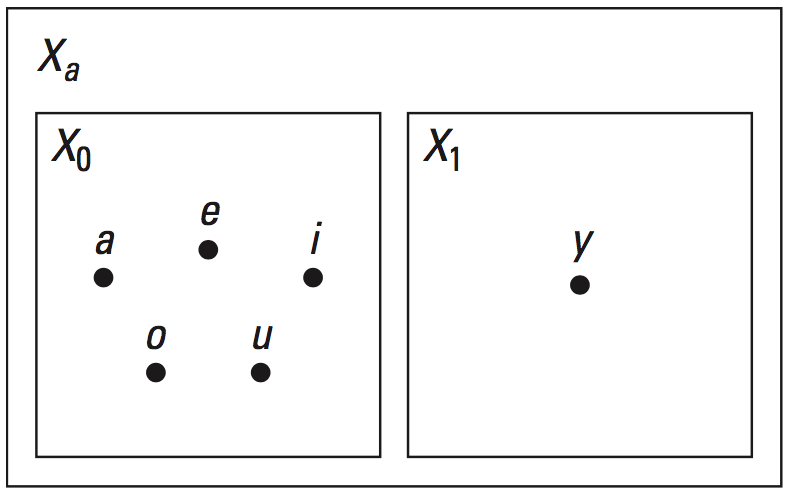
\includegraphics[width=0.5\textwidth]{img/f4-2.png}
            \caption{Figura representativa do mapeamento da aplicação.}
            \label{fig:parti_alfabeto}
        \end{figure}
        %\end{commaent}
\end{comment}
        Com isso, é possível aplicar o formalismo à $ \mathcal{A} $.
        Assumindo que o universo é o conjunto de todas tarefas $B$ de um dispositivo \wearable, então $U$ é as partições de tarefas
        %
        \begin{equation}
            U = \bigcup_{C \in \mathcal{C}} B(C) \label{eq:bigcup}
        \end{equation}
        %
        sendo esta a partição original da aplicação totalmente em \software,\ onde
        %
        \begin{equation}
            \mathcal{S}  = \left \{
            \underbrace{\left \{ b_0, b_1, \dots b_{i-1} \right \}}_{\text{tarefa }C_0},
            \underbrace{\left \{ b_i, b_{i+1}, \dots \right \}}_{\text{tarefa }C_1},\dots
            \underbrace{\left \{ b_j, b_{j+1}, \dots \right \}}_{\text{tarefa }C_{n-1}}
            \right \}
        \end{equation}
        %
        O propósito é a reorganização do conjunto $ U $ e então mapeá-los em $ \mathcal{S} = \left\{S_0, S_1\right\} $ na qual representam os níveis \hs.
        Dessa forma, tem-se uma nova partição $ \mathcal{S}' $ gerando uma nova aplicação $ \mathcal{A}’ = (\mathcal{C}’, \mathcal{L}’) $, inferida a partir da reorganização da partição $ \mathcal{S} $.
        
        Assim, deve-se mapear cada subconjunto de $ \mathcal{S}' $ para ambos \hs,\ como é exibido abaixo
        %
        \begin{equation}
            \mathcal{X}'   = \left \{
            \underbrace{
               \underbrace{
                  \left \{ b_j, b_{j+1}, \dots b_{k-1} \right \}
               }_{\text{tarefa }C_q}
               \underbrace{
                  \left \{ b_k, b_{k+1}, \dots \right \}
               }_{\text{tarefa }C_r}
               \dots
            }_{\text{\software}};
            \
            \underbrace{
               \underbrace{
                  \left \{ b_0, b_1, \dots, b_{i-1} \right \}
               }_{\text{tarefa }C_0}
               \underbrace{
                  \left \{ b_i, b_{i+1}, \dots b_{j-1} \right \}
               }_{\text{tarefa }C_p}
               \dots
            }_{\text{\hardware}}
            \right \} \label{eq:part_final}
        \end{equation}


    \section{Desempenho como Guia ao Particionamento} \label{sec:ganho_desempenho}
        \subsection{Ganho de Desempenho}
        
        Diferente do mundo \software\ onde se tem análise de ordem de complexidade das aplicações, em \hardware\ não possui-se um guia geral para comparação.
        
        
        % y é speedup
        O ganho ao comparar uma solução \hs\ contra uma solução puramente \software, é tipicamente mensurado como \speedup\ representado por $ \gamma $.
        Isso permite comparar recursos contra outros para determinar melhores desempenhos, exibido na Equação \ref{eq:soft_hard}.
        %
        \begin{equation}
             \gamma =
             \frac{
                \text{\textit{hardware speed}}
             }{
                \text{\textit{software speed}}
             }
             =
             \frac{
                \frac{
                   1
                } {
                   \text{\textit{hardware time}}
                }
             } {
                \frac{
                   1
                }{
                   \text{\textit{software time}}
                }
             }
             =
             \frac{
                \text{\textit{software time}}
             } {
                \text{\textit{hardware time}} \label{eq:soft_hard}
             }
        \end{equation}
        
        Dessa forma é possível comparar aplicações totalmente em nível de \software\ com aplicação que utilizam recursos em \hardware.
        Para que o algoritmo em nível de \hardware\ tenha maior desempenho, deseja-se que $ \gamma > 1 $.
        
        \begin{comment}
        %
        Mais especificamente, interessa-se no ganho de desempenho individual de cada recurso e assim, definindo $ \gamma(i), i \in \mathcal{C} $
        %
        \begin{equation}
            \gamma(i) = \frac{s(i)}{h(i) + m(i)}
        \end{equation}
        %
        onde $ h(i) $ e $ s(i) $ são o tempo de execução de uma implementação de um recurso $ i $ em \hs\ e a função $ m(i) $ é o tempo que se leva para sincronização, ou seja, o tempo que leva para guiar um dado entre o processador e o item reconfigurável.
        
        %Assumindo por um momento que usaremos esse recurso separado em nosso \design, deve-se questionar sobre o quão rápido é a aplicação.
        A velocidade da aplicação é dependente dos ganhos de desempenho do recurso e o quão frequentemente ele é utilizado no \design\ referencial de \software.
        Pode-se ter essa fração do tempo gerado de um recurso particular $ p(i) $ a partir de informações de \textit{profile} e dessa forma o \speedup\ da aplicação no geral será
        %
        \begin{equation}
             \Gamma = \left [
             (1 - p(i))
             +
             \frac{
                p(i)
             }{
                \gamma(i)
             } \right ]^{-1}
        \end{equation}
        %
        A inversão representa que estamos movendo entre taxa de execução e tempo de execução para manter o sentido de ganho de desempenho.
        
        A partir dessa equação, podemos observar que aumentando a velocidade do \hardware\ de um único recurso tem-se menos e menos impacto no desempenho da aplicação a medida que sua frequência decresce.
        
        Assim, para aumentar o desempenho sistêmico de uma aplicação no geral, também deve-se aumentar o sistema com múltiplos recursos que aumentará o desempenho de componentes individualmente assim como aumentando a fração agregada de tempo gasto em \hardware.
        Para computar o \speedup\ de múltiplos recursos em \hardware, ou seja, avaliar o ganho sistêmico de um conjunto de recursos $ \mathbb{D} $ onde cada membro do conjunto contribui à desempenho do sistema baseado na fração do tempo gasto em cada característica.
        Para estimar o desempenho desta partição, podemos adicionar recursos e rearranjar os termos para ter um ganho de desempenho almejado no geral, assim para o cálculo de desempenho dos recursos, utiliza-se da Equação \ref{eq:d_final}.
        %
        \begin{equation}
             \Gamma (\mathbb{D}) =
             \left [
             1 + \sum _{i \in \mathbb{D}} \left (
             \frac{
                p(i)
             }{
                \gamma(i)
             }-p(i)
             \right)
             \right ]^{-1} \label{eq:d_final}
        \end{equation}
\end{comment}
        
        \subsection{Recursos Finitos em Componentes Eletrônicos} \label{sec:recursos}
        
            Um FPGA terá um valor escalar total $ r_{FPGA} $, que representará o total de números de \luts\ disponíveis.
            Então $ r(i) $ pode ser usado para representar a quantidade de recursos por cada algoritmo $ i $.
            Tem-se que $ \sum_{i \in \mathbb{D}} r(i) < r_{FPGA} $ restringe quão largo $ \mathbb{D} $ pode crescer, onde $ \mathbb{D} $ é o conjunto de tecnologias em \hardware\ usados para a realização dos algoritmos candidatos.
            
            Uma típica plataforma FPGA tem múltiplos tipos de recursos além de \luts\ como memória, blocos DSP, etc., sendo a quantidade de recursos de cada tecnologia representados matematicamente por
            %
            \begin{equation}
                \vec{r}_{FPGA} =
                \begin{pmatrix}
                r_{Logic\ Cells} \\
                r_{Memory}\\
                r_{DSP}\\
                \vdots \\
                r_{n-1}
                \end{pmatrix}
            \end{equation}
            %
            e com isso,
            %
            %\begin{equation}
            %    \sum_{i \in \mathbb{D}} \vec{r}(i) < \vec{r}_{FPGA}
            %\end{equation}
            %
            $ \sum_{i \in \mathbb{D}} \vec{r}(i) < \vec{r}_{FPGA} $.

    \section{Avaliação do \Wearable}
        Enquanto o desempenho do \wearable\ é avaliado pelo tempo de execução do sistema segundo a Equação \ref{eq:soft_hard}, a alocação de recursos deve ser analisada, tanto em cada um dos \hardwares\ dos algoritmos gerados por HLS, quanto para o sistema como um todo, respeitando o limite de recursos $ \vec{r}_{FPGA} $.
        
        Dessa forma, será utilizado \A$ _i $ para descrever separadamente as implementações dos $ i $ algoritmos candidatos e \Ss$ _j $ referencia-se às implementações dos $ j $ sistemas sintetizados.
        Com a diferenciação entre \A$ _i $ e \Ss$ _j $ (parte e todo do sistema) é possível analisar tanto as implementações dos módulos gerados por HLS separadamente, quanto os sistemas finais na alocação de recursos do FPGA.

        
    \begin{comment}
%\chapter{O Particionamento de \HS\ para Sistemas \Wearable} \label{chap:desenvolvimento}
    \section{O Particionamento de \HS\ para Sistemas \Wearable} \label{sec:desenvolvimento}

        De início, será considerado como aplicação \wearable\ um conjunto de instruções organizadas, e como visto na Seção \ref{sec:gc}, esta também representada por uma coleção de grafos de controle de fluxo, ou seja, grafo de chamada, especificando a sua ordem de execução.
        A partir deste, será feito análises a fim da procura de um particionamento que atenda aos requisitos de dispositivos \wearables, como alto poder de processamento sem o \textit{trade-off} de energia, além de miniaturização, confiabilidade e outros.
        
        Após esclarecidos algumas definições prévias (Seção~\ref{sec:definicoes_previas}), será apresentado o problema na Seção~\ref{sec:declaracao_problema}.
        %Alguns fatores podem ajudar nas decisões de particionamento tal como expectativa de ganho de desempenho (Seção \ref{sec:ganho_desempenho}) e os recursos utilizados em \hardware\ (Seção \ref{sec:recursos}).%, a forma na qual são usados e, talvez os mais importantes, quanto de sobrecarga de comunicação a decomposição impõe (Seção \ref{sec:comunicacao}) \todo{deixar?}e dificuldade de implementar um conjunto específico em \hardware\ (Seção \ref{sec:dificuldades}).\todo{organizar}
        
        \subsection{Definições Prévias} \label{sec:definicoes_previas}
            \begin{description}
                \item [Recurso:] grupo conectado de instruções de uma aplicação de \design\ referencial de \software\ `adequado' para uma implementação em \hardware.
                
                O recurso pode variar de um pequeno conjunto de instruções até um modulo de \software\ completo consistente de múltiplas sub-rotinas.
                Como o tamanho dos recursos afetam no desempenho, a decisão de implementação em \hardware\ depende da sua melhoria no sistema por inteiro e mensura-se os recursos utilizados com relação a outros recursos candidatos.
                
                Se determinado que o recurso é vantajoso, então os recursos de implementação em \hardware\ aumentam a arquitetura de \hardware;
                
                \item [Implementação em \hardware:] recurso adicional de uma específica aplicação;
                
                \item [Adequado:] descrevendo de forma mais geral no âmbito de sistemas \wearable, é a definição da situação na qual o projetista do sistema antecipa a percepção de vantagens na implementação em \hardware.
                %Para obter uma boa partição, geralmente deve-se examinar grupos que podem ser maiores ou menores que sub-rotinas definidas pelo programador.
            \end{description}
            
            \begin{comment}
            \begin{figure}[h] \centering
            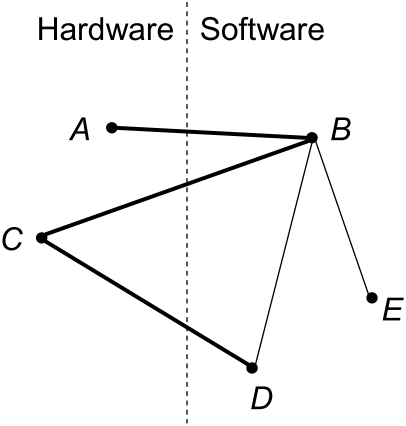
\includegraphics[width=0.4\textwidth]{img/partitioning.png}
            \caption{Representação Geral de um Particionamento em um grafo não direcionado.
            Os $\bullet$ (pontos) representam componentes da aplicação e as --- (linhas) seus respectivos fluxos de comunicação.
            A linha tracejada representa a divisão de níveis entre eles, sendo este \hs.
            Fonte: \citet{Mann2007}.}
            \label{fig:f4-4}
            \end{figure}
            \end{commaent}
            %\section{Declaração Formal do Problema}
            %	Descreveremos problema segundo a definição de \citeauthor{Arato2005, Mann2007} a seguir.
            
            %\section{Solução analítica para particionamento}
            %\section{Visão Analítica Para o Particionamento}
        
        
        \subsection{Declaração do Problema} \label{sec:declaracao_problema}
             Nesta seção serão apresentadas as declarações matemáticas do problema de agrupamento de instruções em recursos e seus mapeamentos em \hardware\ ou \software, ou seja, o particionamento \hs.
             %Segundo \cite{Sass2010}, a forma mais comum de transcrever é descrever manualmente o \core\ com um HDL utilizando \design\ referencial de \software\ como especificação, método utilizado para descrever o problema.
            
             No particionamento, muitos problemas práticos impactam diretamente no desempenho do sistema.
             Nem todos os problemas podem ser incorporados num modelo analítico \cite{Wang2016}, e por isso, só podemos esperar que as soluções matemáticas produzam uma uma resposta aproximada ao problema de particionamento ao utilizar a declaração formal.
            
             Muitas das entradas do modelo são estimadas ou aproximações no qual futuramente degrada a fidelidade de resultados.
             %%Este é um fato relevante pois com isso, resolvendo o problema de particionamento `no papel', tem-se um particionamento que é próximo ao ótimo.
             %%Assim, cabe ao \designer\ ser habilidoso em usar os guias e projetar uma solução mais refinada.
             Dessa forma, é mais eficiente usar uma combinação de técnicas \textit{ad hoc} e matemáticas para encontrar uma solução ótima ou aproximada do que simplesmente confiar numa intuição.
            
            
             %\begin{comment}
             %\section{Declaração do Problema}
             Já descrito as ferramentas matemáticas necessárias para descrever o problema fundamental do particionamento no Capítulo \ref{chap:revisao_bibliografica}, pode-se então descrever formalmente o problema em termos de variáveis. % e descrever um algoritmo \todo{algorit?}para encontrar uma solução aproximada.
             %
             A ideia básica consiste em encontrar um particionamento para todos os blocos básicos de uma aplicação e então separá-los em \hs.
             Formalmente, procura-se por uma partição $ \mathcal{P} $ de todos os blocos básicos $ U $ de uma aplicação (Equação \ref{eq:bigcup}).
             %
             %$$ U = \bigcup_{C \in \mathcal{C}} B(C) $$
             %
             %$ C = (B,F) $
             Definida a partição e o universo, tem-se então um subconjunto $ \mathbb{C}\ |\ \mathbb{C} \subseteq U $, onde $ C \in \mathcal{C} $ é um vértice de um grafo de \design\ referencial de \software\ $ \mathcal{A} = (\mathcal{C}, \mathcal{L}) $ (oriundo da Equação \ref{eq:a}).
             O conjunto $ \mathbb{C} $, chamado conjunto de candidatos, contém todos os recursos arquiteturais potenciais, ou seja, o subconjunto de $ U $ que é esperado para melhorar o desempenho do sistema se implementado em um \hardware\ reconfigurável.
             Devido ao limite de recursos, deve-se refinar para o subconjunto $ \mathbb{D} \subseteq \mathbb{C} $ que maximiza nosso métrica de desempenho.
             Assim
             \begin{equation}
                \begin{array}{rrcl}
                \text{max}                 & \Gamma ( \mathbb{D})               & ~   & ~                \\
                subject\ to & \sum_{i \in \mathbb{D}} \vec{r}(i) & < & \vec{r}_{FPGA}
                \end{array}
                \label{eq:constraints}
             \end{equation}
             %
             Descrevendo algoritmicamente, uma abordagem seria encontrar todas as partições de $ U $, sintetizando e \textit{profiling} cada partição, e então, quantitativamente avaliar cada $ \Gamma $.
             Entretanto, este é um problema linear inteiro devido à natureza de alocação e utilização dos recurso físicos do FPGA. %(Seção \ref{sec:pli})
            
             A seguir, será descrito como é feito uma abordagem para tal, seguindo estudos de \citet{Arato2003, Wang2016}.
        
        \begin{comment}

      \subsection{Abordagem Heurística}
         O problema de particionamento é essencialmente uma questão indireta de manipulação de parâmetros $ p(i) $ e $ \gamma(i) $ (tempo gasto em e ganho de desempenho, respectivamente) pelo rearranjo do particionamento $ \mathcal{X} $.
         Então seleciona-se os elementos de $ \mathcal{X} $ que satisfaz as restrições de recurso e maximiza o desempenho do sistema $ \Gamma $, Equação \ref{eq:constraints}.

         Uma metodologia heurística que pode ser aplicada seria iniciar a partição natural provida pelo \design\ referencial de \software, ou seja, utiliza-se as sub-rotinas de uma aplicação original.
         %
         Utilizando a ferramenta de \textit{profiling}, lista-se as sub-rotinas em ordem decrescente em tempo e verifica-se as que possuem maior valor $ p $.
         O valor de $ \gamma $ será estimado pelo desempenho esperada a partir da implementação em \hardware\ e ao final, tem-se um ganho estimado do sistema para cada sub-rotina.

         Em seguida, quer-se manipular iterativamente a partição $ \mathcal{X} = \{ X_0, X_1, X_2, ...\} $ criando um novo subconjunto de blocos básicos por meio de operações de casamento e movimentações de blocos.
         A ideia em realizar alterações iterativas é encontrar mudanças que podem alterar os valores da fração $ p $ ou o valor de $ \gamma $.

         Num \wearable\ que tenha como procedimentos cálculos matemáticos, verificar quais funções possui maior impacto na sua execução e assim, realizar uma busca a fim de encontrar uma partição de procedimentos que poderiam ser implementados em um acelerador aumentando possivelmente o \speedup\ do sistema.

         Para aumentar o ganho desempenho de recurso $ \gamma (i) $ utilizando abordagens heurísticas, necessita-se verificar o grafo de controle de fluxo do recurso e avaliar se uma mudança o tornará mais sequencial ou paralelo.

         Uma forma de reduzir a fração de tempo gasta de uma sub-rotina é torná-la maior na quantidade de recurso alocada a ela.
         Por exemplo, casando vários blocos básicos num único bloco.
         Isso pode ser alcançado procurando por relações no grafo de chamadas ou, após a manipulação, por relacionamentos no grafo de controle de fluxo que conecta subconjuntos.

         %Frequentemente, algoritmos que são inerentemente sequenciais, ou seja, uma forte dependência em seu fluxo ou dependências de controle, possuem melhor desempenho em processadores, por este não ter a sobrecarga de configurações de transistores e de possuírem melhor gerenciamento de energia nessas circunstâncias.
         %Ou seja, simplesmente adicionar blocos básicos a qualquer custo pode ter um efeito indesejável de aumentar o comportamento sequencial do recurso, reduzindo o valor de $ \gamma $.
         %Entretanto, se um componente utilizar-se de menos recursos, então possui potencial de aumentar seu ganho de desempenho pela simplicidade.

         Exemplificando de uma forma mais abstrata, considera-se uma sub-rotina $ X $ e quebrando-a em duas sob-rotinas $ X – X' $ e $ X' $, onde a sub-rotina $ X – X' $ invoca $ X' $.
         Então se $ X' $ extrai partes de $ X $ que podem ser melhoradas em nível de \hardware\ deixando a parte sequencial em $ X – X' $, então $ \gamma $ de $ X' $ será maior que $ \gamma $ de $ X $ original e provavelmente necessitará de menos recursos.

         %A lei de Ahmdal tenta sempre aumentar a fração de tempo gasto na porção de código que acaba de ser melhorada.
         %No entanto, quando limitado os recursos, nem sempre é melhor.

         Com isso, é importante notar que qualquer mudança no subconjunto pode afetar o desempenho para melhor ou pior.
         Em geral, heurísticas trabalham examinando os grafos da aplicação e então fazendo alterações incrementais ao subconjunto de uma partição.
         Tais mudanças são guiadas pela tentativa de diminuir o tempo gasto em uma sub-rotina não aumentando dramaticamente seus recursos ou decrescendo suo desempenho; e a tentativa de melhorar o desempenho sem aumentar o tempo gasto em uma sub-rotina.

\end{commaent}


   %\section{Metodologia Proposta}
    \section{Proposta de Procedimento Analítico} \label{sec:proposta}

        Como conclusão deste capítulo, será formulada uma proposta de metodologia analítica baseada nos conceitos propostos pela literatura, com o foco em componentes procedurais integrados à sistemas \wearables.
        %E com isso, o trabalho consiste em desenvolver seus respectivos grafos e realizar o particionamento a fim de encontrar uma solução aproximada, respeitando os seus requisitos de funcionamento.
        %
        Tal metodologia, apresentada pelo Algoritmo~\ref{alg:proposta}, será considerada apenas como uma orientação para os passos a serem realizados, sendo então, uma proposta representativa do processo a ser realizado para a análise e decisão de particionamento.

      \begin{algorithm}[h]
         \SetKwData{itt}{it}
         \SetKwData{pl}{partition\_list}
         \SetKwData{complexSet}{how\_complex\_set\_is}
         \SetKwData{md}{matriz\_dados}
         \SetKwData{complexSet}{how\_complex\_set\_is}
         \SetKwFunction{graph}{makes\_graph}
         \SetKwFunction{porte}{analyses\_complex\_set}
         \SetKwFunction{synth}{synthesizes}
         \SetKwFunction{resources}{resources\_used}
         \SetKwFunction{die}{die\_used}
         \SetKwFunction{energy}{energy\_spent}
         \SetKwFunction{profiling}{profile}
         \SetKwFunction{desempenho}{desempenho\_analysis}
         \SetKwFunction{factor}{complexity\_factor}
         \SetKwFunction{ilp}{integer\_linear\_solve}
         \SetKwFunction{heuristic}{heuristic}
         \KwIn{a project description.}
         \KwOut{a partition solved.}

         %\BlankLine
         \Begin{

            \BlankLine
            \profiling{}\;
            \BlankLine

            \tcp{extration project analyses}
            \graph{Flow Control Graph}\;
            \graph{Call Graph}\;
            %\complexSet $\leftarrow$ \porte{}\tcp*{verify if it is a big project}

            \BlankLine

            \If{exist partitions that can be synthesized}{
               \ForEach{partition project:\itt $\in$ \pl}{
                  \synth{\itt}\;
                  \BlankLine
                  \resources{\itt}\tcp*{analysis after synth}
                  \die{\itt}\;
                  \energy{\itt}\;
                  %\BlankLine


                  \desempenho{\itt}\;
               }
               \BlankLine

               %\uIf(\tcp*[f]{verify if it is a small project}){\factor{\complexSet}}{
                  \ilp{\pl}\tcp*{analyse quantitatively each $ \Gamma $}
               %}
               %\lElse{
                  %\heuristic{\pl}\;
               %}
            }
         }
         \caption{Metodologia para avaliação de \wearables.}
         \label{alg:proposta}
      \end{algorithm}

        Apresentado o procedimento metodológico, a seguir será listada cada função pertencente à metodologia acima, descrevendo suas funções e seu propósito no trabalho para a obtenção dos objetivos.
        Para um melhor compreendimento, serão divididos em quatro seções, sendo elas: visualização do projeto, síntese, análise de síntese, particionamento.

      \begin{comment}
      Dessa forma, o primeiro passo proposto é a análise do sistema por meio de testes em nível de \software, ou seja, o sistema realizado sobre um processador.
      Como exibido no Algoritmo~\ref{alg:manual}, os processos se baseiam na construção e análise do sistema em um processador.
      Deve-se realizar a construção de seus gráficos para seu entendimento (linhas 2 e 3), e em seguida (linha 4) uma avaliação do porte do sistema, item essencial para a escolha do algoritmo propício ao realizar o particionamento, caso exista.
      Nas linhas 5, 6 e 7 são análises feitas a partir da execução do mesmo numa plataforma, obtendo seu \profile, desempenho e gasto energético respectivamente.

      \begin{algorithm}[h]
        %\KwResult{Write ere the result }
        \SetKwData{md}{matriz\_dados}
        \SetKwData{complexSet}{how\_complex\_set\_is}
        \SetKwFunction{graph}{makes\_graph}
        \SetKwFunction{porte}{analyses\_complex\_set}
        \SetKwFunction{energy}{energy\_spent\_analyses}
        \SetKwFunction{desempenho}{desempenho\_analyses}
        \SetKwFunction{profiling}{profile}
        \KwIn{software reference design.}
        \KwOut{software analyses.}
        \BlankLine
        \tcc{this algorithm happens in a soft core system without anyone accelearator}
        \BlankLine
        \Begin{

           \tcp{extration project analyses}
           \graph{Flow Control Graph}\;
           \graph{Call Graph}\;
           \complexSet $\leftarrow$ \porte{}\tcp*{verify if it is a big project}

           \BlankLine

           \tcp{physical project analyses}
           \profiling{}\;
           \desempenho{}\;
           \energy{}\;
        }
        \caption{Processos manuais para análise inicial do dispositivo.}
        \label{alg:manual}
      \end{algorithm}
\end{commeant}


        \begin{enumerate}
            \item Procedimentos para visualização geral do projeto.
            Por meio dos dados do \profile\ e a construção dos grafos, é possível ter uma visão geral, verificando se o sistema possui possíveis seções de processamentos críticos para a realização de particionamento \hs.
            As funções presentes são:
            
            \begin{itemize}
                \item \texttt{profile():}
                procedimento referente à Seção~\ref{sec:profile}.
                Realiza-se uma análise de tempo gasto em cada procedimento do projeto, apresentando-a ao final de sua execução.
                Com os resultados, é possível ver locais onde existe um tempo maior de processamento gasto ou de recursos utilizados indicando uma verificação detalhada sobre este a fim de candidatá-lo para uma implementação em \hardware;
                
                \item \texttt{makes\_graph(}\textit{type}\texttt{):}
                constrói-se grafos relativos ao projeto, sendo estes de acordo com o tipo especificado no parâmetro.
                A construção do grafo segue como descrito na Seção~\ref{sec:GCF} na qual procura-se por seções de códigos compondo-os em blocos, compreendendo o fluxo do algoritmo e consecutivamente os procedimentos de chamadas.
                O parâmetro simboliza a especificação de qual tipo de grafo será construído, sendo ele um grafo de controle de fluxo (Seção~\ref{sec:GCF}) ou grafo de chamada (Seção~\ref{sec:gc}), que como já explicado, necessita do anterior para sua construção;
            \end{itemize}
            
            \item \texttt{synthesizes():}
            caso exista uma possibilidade de particionamento, análise obtida pelo \profile, visualização do grafo e obtenção de uma lista de candidatos, realiza-se então o procedimento de geração de HDL para o desenvolvimento de aceleradores em \textit{hardware} reconfigurável e sua análise de desempenho e gastos tanto de energia quanto de recursos;
            
            \item Após a execução do processo de síntese realizado junto com a ferramenta sintetizadora assistida pelo computador, é possível obter vários dados analíticos de alocação de recursos como quantidade de elementos lógicos utilizados, pinos virtuais e físicos, quantidade de bits de memória, além de vários outros.
            E com a sua sintetização na plataforma, também é possível obter a avaliação de consumo energético, \profile\ e desempenho.
            Estes são representados pelos métodos abaixo na qual, aplica-se a cada componente sintetizado separadamente.
            \begin{itemize}
            
                \item \texttt{resources\_used():}
                quais e a quantidade de recursos alocados para utilização no projeto de geração de aceleradores.
                A alocação de muitos recursos implica num gasto maior de energia criando um \textit{trade-off} a ser analisado;
                
                \item \texttt{die\_used():}
                tamanho do \textit{die} utilizado para o projeto do acelerador.
                Sistemas \wearable\ possuem como requisito a sua miniaturização, impedindo que seu uso limite a capacidade de locomoção, usabilidade ou conforto do usuário, por exemplo;
                
                \item \texttt{energy\_spent():}
                valores energéticos do uso do recurso implementado, incluindo os módulos pertencentes a ele como memórias, DSPs e quaisquer outros que estejam integrados à plataforma;
                
                \item \texttt{desempenho\_analysis():}
                comparação das implementações em \hardware\ sobre os recursos em nível de \textit{software}, ou seja análise de desempenho.
            \end{itemize}
            
            \item \texttt{integer\_linear\_solver():}
            após realizado todas as análises individuais acima, inicia-se o processo de procura de uma solução de particionamento que obtenha bons resultados nos requisitos de um sistema \wearable.
            Dessa forma, é realizado uma avaliação por meio de um \textit{solver} linear inteiro segundo os dados obtidos.
            Com o \textit{solver}, é possível realizar uma busca a procura de um particionamento que atenda a quantidade máxima de restrições exigidas por um \wearable.
        \end{enumerate}
        
        
        %Conclusão
        Assim, o trabalho consiste numa metodologia na qual aborda o particionamento para dispositivos \wearables, partindo de uma análise de execução do \software, candidatando alguns procedimentos para sua sintetização e assim a avaliação destes segundo os recursos utilizados para a completude de suas tarefas o que chamamos de particionamento, consistindo da procura de um conjunto que traga melhor desempenho no seu uso. Tudo isso, utilizando recursos disponibilizados pela plataforma em \hardware.
        %O Algoritmo~\ref{alg:proposta} tem como o objetivo a demonstração do passos necessários para o compreendimento do sistema a ser analisado e consecutivamente a sua partição em busca do aprimoramento da seu desempenho.
\end{comment}